\documentclass[1p]{elsarticle_modified}
%\bibliographystyle{elsarticle-num}

%\usepackage[colorlinks]{hyperref}
%\usepackage{abbrmath_seonhwa} %\Abb, \Ascr, \Acal ,\Abf, \Afrak
\usepackage{amsfonts}
\usepackage{amssymb}
\usepackage{amsmath}
\usepackage{amsthm}
\usepackage{scalefnt}
\usepackage{amsbsy}
\usepackage{kotex}
\usepackage{caption}
\usepackage{subfig}
\usepackage{color}
\usepackage{graphicx}
\usepackage{xcolor} %% white, black, red, green, blue, cyan, magenta, yellow
\usepackage{float}
\usepackage{setspace}
\usepackage{hyperref}

\usepackage{tikz}
\usetikzlibrary{arrows}

\usepackage{multirow}
\usepackage{array} % fixed length table
\usepackage{hhline}

%%%%%%%%%%%%%%%%%%%%%
\makeatletter
\renewcommand*\env@matrix[1][\arraystretch]{%
	\edef\arraystretch{#1}%
	\hskip -\arraycolsep
	\let\@ifnextchar\new@ifnextchar
	\array{*\c@MaxMatrixCols c}}
\makeatother %https://tex.stackexchange.com/questions/14071/how-can-i-increase-the-line-spacing-in-a-matrix
%%%%%%%%%%%%%%%

\usepackage[normalem]{ulem}

\newcommand{\msout}[1]{\ifmmode\text{\sout{\ensuremath{#1}}}\else\sout{#1}\fi}
%SOURCE: \msout is \stkout macro in https://tex.stackexchange.com/questions/20609/strikeout-in-math-mode

\newcommand{\cancel}[1]{
	\ifmmode
	{\color{red}\msout{#1}}
	\else
	{\color{red}\sout{#1}}
	\fi
}

\newcommand{\add}[1]{
	{\color{blue}\uwave{#1}}
}

\newcommand{\replace}[2]{
	\ifmmode
	{\color{red}\msout{#1}}{\color{blue}\uwave{#2}}
	\else
	{\color{red}\sout{#1}}{\color{blue}\uwave{#2}}
	\fi
}

\newcommand{\Sol}{\mathcal{S}} %segment
\newcommand{\D}{D} %diagram
\newcommand{\A}{\mathcal{A}} %arc


%%%%%%%%%%%%%%%%%%%%%%%%%%%%%5 test

\def\sl{\operatorname{\textup{SL}}(2,\Cbb)}
\def\psl{\operatorname{\textup{PSL}}(2,\Cbb)}
\def\quan{\mkern 1mu \triangleright \mkern 1mu}

\theoremstyle{definition}
\newtheorem{thm}{Theorem}[section]
\newtheorem{prop}[thm]{Proposition}
\newtheorem{lem}[thm]{Lemma}
\newtheorem{ques}[thm]{Question}
\newtheorem{cor}[thm]{Corollary}
\newtheorem{defn}[thm]{Definition}
\newtheorem{exam}[thm]{Example}
\newtheorem{rmk}[thm]{Remark}
\newtheorem{alg}[thm]{Algorithm}

\newcommand{\I}{\sqrt{-1}}
\begin{document}

%\begin{frontmatter}
%
%\title{Boundary parabolic representations of knots up to 8 crossings}
%
%%% Group authors per affiliation:
%\author{Yunhi Cho} 
%\address{Department of Mathematics, University of Seoul, Seoul, Korea}
%\ead{yhcho@uos.ac.kr}
%
%
%\author{Seonhwa Kim} %\fnref{s_kim}}
%\address{Center for Geometry and Physics, Institute for Basic Science, Pohang, 37673, Korea}
%\ead{ryeona17@ibs.re.kr}
%
%\author{Hyuk Kim}
%\address{Department of Mathematical Sciences, Seoul National University, Seoul 08826, Korea}
%\ead{hyukkim@snu.ac.kr}
%
%\author{Seokbeom Yoon}
%\address{Department of Mathematical Sciences, Seoul National University, Seoul, 08826,  Korea}
%\ead{sbyoon15@snu.ac.kr}
%
%\begin{abstract}
%We find all boundary parabolic representation of knots up to 8 crossings.
%
%\end{abstract}
%\begin{keyword}
%    \MSC[2010] 57M25 
%\end{keyword}
%
%\end{frontmatter}

%\linenumbers
%\tableofcontents
%
\newcommand\colored[1]{\textcolor{white}{\rule[-0.35ex]{0.8em}{1.4ex}}\kern-0.8em\color{red} #1}%
%\newcommand\colored[1]{\textcolor{white}{ #1}\kern-2.17ex	\textcolor{white}{ #1}\kern-1.81ex	\textcolor{white}{ #1}\kern-2.15ex\color{red}#1	}

{\Large $\underline{12a_{0048}~(K12a_{0048})}$}

\setlength{\tabcolsep}{10pt}
\renewcommand{\arraystretch}{1.6}
\vspace{1cm}\begin{tabular}{m{100pt}>{\centering\arraybackslash}m{274pt}}
\multirow{5}{120pt}{
	\centering
	\includegraphics[width=112pt]{../../../GIT/diagram.site/Diagrams/png/849_12a_0048.png}\\
\ \ \ A knot diagram\footnotemark}&
\allowdisplaybreaks
\textbf{Linearized knot diagam} \\
\cline{2-2}
 &
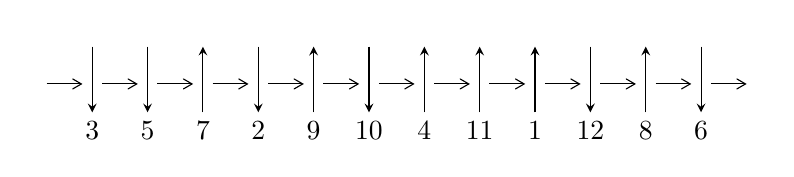
\begin{tikzpicture}[x=20pt, y=17pt]
	% nodes
	\node (C0) at (0, 0) {};
	\node (C1) at (1, 0) {};
	\node (C1U) at (1, +1) {};
	\node (C1D) at (1, -1) {3};

	\node (C2) at (2, 0) {};
	\node (C2U) at (2, +1) {};
	\node (C2D) at (2, -1) {5};

	\node (C3) at (3, 0) {};
	\node (C3U) at (3, +1) {};
	\node (C3D) at (3, -1) {7};

	\node (C4) at (4, 0) {};
	\node (C4U) at (4, +1) {};
	\node (C4D) at (4, -1) {2};

	\node (C5) at (5, 0) {};
	\node (C5U) at (5, +1) {};
	\node (C5D) at (5, -1) {9};

	\node (C6) at (6, 0) {};
	\node (C6U) at (6, +1) {};
	\node (C6D) at (6, -1) {10};

	\node (C7) at (7, 0) {};
	\node (C7U) at (7, +1) {};
	\node (C7D) at (7, -1) {4};

	\node (C8) at (8, 0) {};
	\node (C8U) at (8, +1) {};
	\node (C8D) at (8, -1) {11};

	\node (C9) at (9, 0) {};
	\node (C9U) at (9, +1) {};
	\node (C9D) at (9, -1) {1};

	\node (C10) at (10, 0) {};
	\node (C10U) at (10, +1) {};
	\node (C10D) at (10, -1) {12};

	\node (C11) at (11, 0) {};
	\node (C11U) at (11, +1) {};
	\node (C11D) at (11, -1) {8};

	\node (C12) at (12, 0) {};
	\node (C12U) at (12, +1) {};
	\node (C12D) at (12, -1) {6};
	\node (C13) at (13, 0) {};

	% arrows
	\draw[->,>={angle 60}]
	(C0) edge (C1) (C1) edge (C2) (C2) edge (C3) (C3) edge (C4) (C4) edge (C5) (C5) edge (C6) (C6) edge (C7) (C7) edge (C8) (C8) edge (C9) (C9) edge (C10) (C10) edge (C11) (C11) edge (C12) (C12) edge (C13) ;	\draw[->,>=stealth]
	(C1U) edge (C1D) (C2U) edge (C2D) (C3D) edge (C3U) (C4U) edge (C4D) (C5D) edge (C5U) (C6U) edge (C6D) (C7D) edge (C7U) (C8D) edge (C8U) (C9D) edge (C9U) (C10U) edge (C10D) (C11D) edge (C11U) (C12U) edge (C12D) ;
	\end{tikzpicture} \\
\hhline{~~} \\& 
\textbf{Solving Sequence} \\ \cline{2-2} 
 &
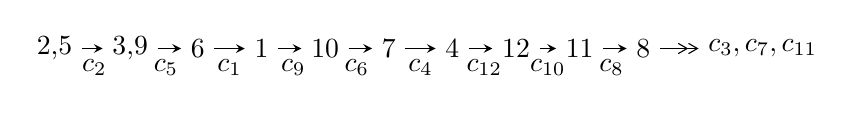
\begin{tikzpicture}[x=23pt, y=7pt]
	% node
	\node (A0) at (-1/8, 0) {2,5};
	\node (A1) at (17/16, 0) {3,9};
	\node (A2) at (17/8, 0) {6};
	\node (A3) at (25/8, 0) {1};
	\node (A4) at (33/8, 0) {10};
	\node (A5) at (41/8, 0) {7};
	\node (A6) at (49/8, 0) {4};
	\node (A7) at (57/8, 0) {12};
	\node (A8) at (65/8, 0) {11};
	\node (A9) at (73/8, 0) {8};
	\node (C1) at (1/2, -1) {$c_{2}$};
	\node (C2) at (13/8, -1) {$c_{5}$};
	\node (C3) at (21/8, -1) {$c_{1}$};
	\node (C4) at (29/8, -1) {$c_{9}$};
	\node (C5) at (37/8, -1) {$c_{6}$};
	\node (C6) at (45/8, -1) {$c_{4}$};
	\node (C7) at (53/8, -1) {$c_{12}$};
	\node (C8) at (61/8, -1) {$c_{10}$};
	\node (C9) at (69/8, -1) {$c_{8}$};
	\node (A10) at (11, 0) {$c_{3},c_{7},c_{11}$};

	% edge
	\draw[->,>=stealth]	
	(A0) edge (A1) (A1) edge (A2) (A2) edge (A3) (A3) edge (A4) (A4) edge (A5) (A5) edge (A6) (A6) edge (A7) (A7) edge (A8) (A8) edge (A9) ;
	\draw[->>,>={angle 60}]	
	(A9) edge (A10);
\end{tikzpicture} \\ 

\end{tabular} \\

\footnotetext{
The image of knot diagram is generated by the software ``\textbf{Draw programme}" developed by Andrew Bartholomew(\url{http://www.layer8.co.uk/maths/draw/index.htm\#Running-draw}), where we modified some parts for our purpose(\url{https://github.com/CATsTAILs/LinksPainter}).
}\phantom \\ \newline 
\centering \textbf{Ideals for irreducible components\footnotemark of $X_{\text{par}}$} 
 
\begin{align*}
I^u_{1}&=\langle 
5.88695\times10^{226} u^{139}+3.54230\times10^{227} u^{138}+\cdots+2.19679\times10^{225} b-1.39977\times10^{227},\\
\phantom{I^u_{1}}&\phantom{= \langle  }-1.53329\times10^{227} u^{139}-1.75240\times10^{228} u^{138}+\cdots+2.19679\times10^{225} a-5.19955\times10^{227},\\
\phantom{I^u_{1}}&\phantom{= \langle  }u^{140}+11 u^{139}+\cdots+5 u+1\rangle \\
I^u_{2}&=\langle 
a^3+a^2+b,\;a^4+a^2- a+1,\;u-1\rangle \\
I^u_{3}&=\langle 
3 a^5+a^4+5 a^3+3 a^2+b+2 a+4,\;a^6+a^5+2 a^4+2 a^3+2 a^2+2 a+1,\;u-1\rangle \\
\\
\end{align*}
\raggedright * 3 irreducible components of $\dim_{\mathbb{C}}=0$, with total 150 representations.\\
\footnotetext{All coefficients of polynomials are rational numbers. But the coefficients are sometimes approximated in decimal forms when there is not enough margin.}
\newpage
\renewcommand{\arraystretch}{1}
\centering \section*{I. $I^u_{1}= \langle 5.89\times10^{226} u^{139}+3.54\times10^{227} u^{138}+\cdots+2.20\times10^{225} b-1.40\times10^{227},\;-1.53\times10^{227} u^{139}-1.75\times10^{228} u^{138}+\cdots+2.20\times10^{225} a-5.20\times10^{227},\;u^{140}+11 u^{139}+\cdots+5 u+1 \rangle$}
\flushleft \textbf{(i) Arc colorings}\\
\begin{tabular}{m{7pt} m{180pt} m{7pt} m{180pt} }
\flushright $a_{2}=$&$\begin{pmatrix}1\\0\end{pmatrix}$ \\
\flushright $a_{5}=$&$\begin{pmatrix}0\\u\end{pmatrix}$ \\
\flushright $a_{3}=$&$\begin{pmatrix}1\\u^2\end{pmatrix}$ \\
\flushright $a_{9}=$&$\begin{pmatrix}69.7967 u^{139}+797.709 u^{138}+\cdots+88.8689 u+236.689\\-26.7979 u^{139}-161.249 u^{138}+\cdots+136.086 u+63.7186\end{pmatrix}$ \\
\flushright $a_{6}=$&$\begin{pmatrix}480.698 u^{139}+4767.03 u^{138}+\cdots+1232.37 u+469.393\\728.821 u^{139}+7333.60 u^{138}+\cdots+2537.70 u+602.691\end{pmatrix}$ \\
\flushright $a_{1}=$&$\begin{pmatrix}- u^2+1\\- u^4\end{pmatrix}$ \\
\flushright $a_{10}=$&$\begin{pmatrix}82.0957 u^{139}+1002.56 u^{138}+\cdots+303.107 u+313.689\\-74.9368 u^{139}-514.534 u^{138}+\cdots+292.890 u+117.321\end{pmatrix}$ \\
\flushright $a_{7}=$&$\begin{pmatrix}-14.2692 u^{139}-127.488 u^{138}+\cdots+14.2050 u-0.190764\\-29.4738 u^{139}-285.330 u^{138}+\cdots-71.1553 u-14.2692\end{pmatrix}$ \\
\flushright $a_{4}=$&$\begin{pmatrix}u\\u\end{pmatrix}$ \\
\flushright $a_{12}=$&$\begin{pmatrix}-201.075 u^{139}-2109.48 u^{138}+\cdots-821.483 u-254.837\\-216.675 u^{139}-2363.19 u^{138}+\cdots-1211.53 u-298.416\end{pmatrix}$ \\
\flushright $a_{11}=$&$\begin{pmatrix}148.855 u^{139}+1559.41 u^{138}+\cdots+437.161 u+239.438\\130.468 u^{139}+1417.38 u^{138}+\cdots+697.783 u+181.413\end{pmatrix}$ \\
\flushright $a_{8}=$&$\begin{pmatrix}-13.2474 u^{139}-129.302 u^{138}+\cdots-17.6313 u-9.59894\\-28.4520 u^{139}-287.145 u^{138}+\cdots-102.992 u-23.6774\end{pmatrix}$\\&\end{tabular}
\flushleft \textbf{(ii) Obstruction class $= -1$}\\~\\
\flushleft \textbf{(iii) Cusp Shapes $= 25.0878 u^{139}-46.6962 u^{138}+\cdots-1004.65 u-85.3740$}\\~\\
\newpage\renewcommand{\arraystretch}{1}
\flushleft \textbf{(iv) u-Polynomials at the component}\newline \\
\begin{tabular}{m{50pt}|m{274pt}}
Crossings & \hspace{64pt}u-Polynomials at each crossing \\
\hline $$\begin{aligned}c_{1}\end{aligned}$$&$\begin{aligned}
&u^{140}+69 u^{139}+\cdots+221 u+1
\end{aligned}$\\
\hline $$\begin{aligned}c_{2},c_{4}\end{aligned}$$&$\begin{aligned}
&u^{140}-11 u^{139}+\cdots-5 u+1
\end{aligned}$\\
\hline $$\begin{aligned}c_{3},c_{7}\end{aligned}$$&$\begin{aligned}
&u^{140}- u^{139}+\cdots-8192 u+1024
\end{aligned}$\\
\hline $$\begin{aligned}c_{5}\end{aligned}$$&$\begin{aligned}
&u^{140}-2 u^{139}+\cdots-24012 u+5887
\end{aligned}$\\
\hline $$\begin{aligned}c_{6}\end{aligned}$$&$\begin{aligned}
&u^{140}+2 u^{139}+\cdots-10624 u+1216
\end{aligned}$\\
\hline $$\begin{aligned}c_{8},c_{11}\end{aligned}$$&$\begin{aligned}
&u^{140}+2 u^{139}+\cdots+14 u+1
\end{aligned}$\\
\hline $$\begin{aligned}c_{9}\end{aligned}$$&$\begin{aligned}
&u^{140}+14 u^{139}+\cdots+2 u+1
\end{aligned}$\\
\hline $$\begin{aligned}c_{10}\end{aligned}$$&$\begin{aligned}
&u^{140}+58 u^{139}+\cdots+14 u+1
\end{aligned}$\\
\hline $$\begin{aligned}c_{12}\end{aligned}$$&$\begin{aligned}
&u^{140}-10 u^{139}+\cdots-2 u+1
\end{aligned}$\\
\hline
\end{tabular}\\~\\
\newpage\renewcommand{\arraystretch}{1}
\flushleft \textbf{(v) Riley Polynomials at the component}\newline \\
\begin{tabular}{m{50pt}|m{274pt}}
Crossings & \hspace{64pt}Riley Polynomials at each crossing \\
\hline $$\begin{aligned}c_{1}\end{aligned}$$&$\begin{aligned}
&y^{140}+15 y^{139}+\cdots-2817 y+1
\end{aligned}$\\
\hline $$\begin{aligned}c_{2},c_{4}\end{aligned}$$&$\begin{aligned}
&y^{140}-69 y^{139}+\cdots-221 y+1
\end{aligned}$\\
\hline $$\begin{aligned}c_{3},c_{7}\end{aligned}$$&$\begin{aligned}
&y^{140}-63 y^{139}+\cdots-25690112 y+1048576
\end{aligned}$\\
\hline $$\begin{aligned}c_{5}\end{aligned}$$&$\begin{aligned}
&y^{140}+142 y^{139}+\cdots+261556046 y+34656769
\end{aligned}$\\
\hline $$\begin{aligned}c_{6}\end{aligned}$$&$\begin{aligned}
&y^{140}+150 y^{139}+\cdots+35716096 y+1478656
\end{aligned}$\\
\hline $$\begin{aligned}c_{8},c_{11}\end{aligned}$$&$\begin{aligned}
&y^{140}+58 y^{139}+\cdots+14 y+1
\end{aligned}$\\
\hline $$\begin{aligned}c_{9}\end{aligned}$$&$\begin{aligned}
&y^{140}+10 y^{139}+\cdots+14 y+1
\end{aligned}$\\
\hline $$\begin{aligned}c_{10}\end{aligned}$$&$\begin{aligned}
&y^{140}+50 y^{139}+\cdots-2010 y+1
\end{aligned}$\\
\hline $$\begin{aligned}c_{12}\end{aligned}$$&$\begin{aligned}
&y^{140}+14 y^{139}+\cdots+10 y+1
\end{aligned}$\\
\hline
\end{tabular}\\~\\
\newpage\flushleft \textbf{(vi) Complex Volumes and Cusp Shapes}
$$\begin{array}{c|c|c}  
\text{Solutions to }I^u_{1}& \I (\text{vol} + \sqrt{-1}CS) & \text{Cusp shape}\\
 \hline 
\begin{aligned}
u &= -0.342968 + 0.929621 I \\
a &= \phantom{-}1.35534 + 0.86261 I \\
b &= -0.303012 - 0.058151 I\end{aligned}
 & \phantom{-}4.92055 - 8.62646 I & \phantom{-0.000000 } 0 \\ \hline\begin{aligned}
u &= -0.342968 - 0.929621 I \\
a &= \phantom{-}1.35534 - 0.86261 I \\
b &= -0.303012 + 0.058151 I\end{aligned}
 & \phantom{-}4.92055 + 8.62646 I & \phantom{-0.000000 } 0 \\ \hline\begin{aligned}
u &= -0.940954 + 0.310093 I \\
a &= -1.00907 + 1.00614 I \\
b &= -0.62230 + 1.81875 I\end{aligned}
 & -1.78233 - 1.83282 I & \phantom{-0.000000 } 0 \\ \hline\begin{aligned}
u &= -0.940954 - 0.310093 I \\
a &= -1.00907 - 1.00614 I \\
b &= -0.62230 - 1.81875 I\end{aligned}
 & -1.78233 + 1.83282 I & \phantom{-0.000000 } 0 \\ \hline\begin{aligned}
u &= -0.982775 + 0.239312 I \\
a &= \phantom{-}0.92340 - 1.08802 I \\
b &= \phantom{-}0.85110 - 1.99683 I\end{aligned}
 & -4.37037 - 6.99484 I & \phantom{-0.000000 } 0 \\ \hline\begin{aligned}
u &= -0.982775 - 0.239312 I \\
a &= \phantom{-}0.92340 + 1.08802 I \\
b &= \phantom{-}0.85110 + 1.99683 I\end{aligned}
 & -4.37037 + 6.99484 I & \phantom{-0.000000 } 0 \\ \hline\begin{aligned}
u &= -0.313843 + 0.961586 I \\
a &= -1.51506 - 0.83479 I \\
b &= \phantom{-}0.480798 + 0.216981 I\end{aligned}
 & \phantom{-}2.9856 - 14.5493 I & \phantom{-0.000000 } 0 \\ \hline\begin{aligned}
u &= -0.313843 - 0.961586 I \\
a &= -1.51506 + 0.83479 I \\
b &= \phantom{-}0.480798 - 0.216981 I\end{aligned}
 & \phantom{-}2.9856 + 14.5493 I & \phantom{-0.000000 } 0 \\ \hline\begin{aligned}
u &= \phantom{-}0.895882 + 0.410358 I \\
a &= \phantom{-}0.737122 - 0.522383 I \\
b &= -1.16839 - 1.04334 I\end{aligned}
 & \phantom{-}0.79500 - 3.33230 I & \phantom{-0.000000 } 0 \\ \hline\begin{aligned}
u &= \phantom{-}0.895882 - 0.410358 I \\
a &= \phantom{-}0.737122 + 0.522383 I \\
b &= -1.16839 + 1.04334 I\end{aligned}
 & \phantom{-}0.79500 + 3.33230 I & \phantom{-0.000000 } 0\\
 \hline 
 \end{array}$$\newpage$$\begin{array}{c|c|c}  
\text{Solutions to }I^u_{1}& \I (\text{vol} + \sqrt{-1}CS) & \text{Cusp shape}\\
 \hline 
\begin{aligned}
u &= \phantom{-}0.928796 + 0.320294 I \\
a &= \phantom{-}0.41566 + 2.57834 I \\
b &= \phantom{-}2.39910 + 3.21755 I\end{aligned}
 & -1.66193 + 0.85450 I & \phantom{-0.000000 } 0 \\ \hline\begin{aligned}
u &= \phantom{-}0.928796 - 0.320294 I \\
a &= \phantom{-}0.41566 - 2.57834 I \\
b &= \phantom{-}2.39910 - 3.21755 I\end{aligned}
 & -1.66193 - 0.85450 I & \phantom{-0.000000 } 0 \\ \hline\begin{aligned}
u &= \phantom{-}0.938441 + 0.410293 I \\
a &= -0.278288 + 0.769078 I \\
b &= \phantom{-}0.432906 + 1.251360 I\end{aligned}
 & -1.82288 - 1.42035 I & \phantom{-0.000000 } 0 \\ \hline\begin{aligned}
u &= \phantom{-}0.938441 - 0.410293 I \\
a &= -0.278288 - 0.769078 I \\
b &= \phantom{-}0.432906 - 1.251360 I\end{aligned}
 & -1.82288 + 1.42035 I & \phantom{-0.000000 } 0 \\ \hline\begin{aligned}
u &= \phantom{-}1.038840 + 0.126611 I \\
a &= \phantom{-}1.02386 + 1.05217 I \\
b &= \phantom{-}6.21349 + 1.31481 I\end{aligned}
 & -2.14003 - 2.45951 I & \phantom{-0.000000 } 0 \\ \hline\begin{aligned}
u &= \phantom{-}1.038840 - 0.126611 I \\
a &= \phantom{-}1.02386 - 1.05217 I \\
b &= \phantom{-}6.21349 - 1.31481 I\end{aligned}
 & -2.14003 + 2.45951 I & \phantom{-0.000000 } 0 \\ \hline\begin{aligned}
u &= -0.980690 + 0.381123 I \\
a &= \phantom{-}0.357441 - 1.087270 I \\
b &= -0.26536 - 1.65226 I\end{aligned}
 & -2.17880 + 4.32767 I & \phantom{-0.000000 } 0 \\ \hline\begin{aligned}
u &= -0.980690 - 0.381123 I \\
a &= \phantom{-}0.357441 + 1.087270 I \\
b &= -0.26536 + 1.65226 I\end{aligned}
 & -2.17880 - 4.32767 I & \phantom{-0.000000 } 0 \\ \hline\begin{aligned}
u &= -0.426331 + 0.962752 I \\
a &= -0.868941 - 0.376457 I \\
b &= \phantom{-}0.138975 + 0.269813 I\end{aligned}
 & \phantom{-}3.40573 - 1.43298 I & \phantom{-0.000000 } 0 \\ \hline\begin{aligned}
u &= -0.426331 - 0.962752 I \\
a &= -0.868941 + 0.376457 I \\
b &= \phantom{-}0.138975 - 0.269813 I\end{aligned}
 & \phantom{-}3.40573 + 1.43298 I & \phantom{-0.000000 } 0\\
 \hline 
 \end{array}$$\newpage$$\begin{array}{c|c|c}  
\text{Solutions to }I^u_{1}& \I (\text{vol} + \sqrt{-1}CS) & \text{Cusp shape}\\
 \hline 
\begin{aligned}
u &= \phantom{-}0.998116 + 0.346400 I \\
a &= -0.89627 - 3.02269 I \\
b &= -3.41213 - 4.72470 I\end{aligned}
 & -1.93443 - 3.19824 I & \phantom{-0.000000 } 0 \\ \hline\begin{aligned}
u &= \phantom{-}0.998116 - 0.346400 I \\
a &= -0.89627 + 3.02269 I \\
b &= -3.41213 + 4.72470 I\end{aligned}
 & -1.93443 + 3.19824 I & \phantom{-0.000000 } 0 \\ \hline\begin{aligned}
u &= -0.902938 + 0.241403 I \\
a &= -0.130518 + 1.318270 I \\
b &= \phantom{-}0.45541 + 1.86743 I\end{aligned}
 & -5.78935 + 0.68606 I & \phantom{-0.000000 } 0 \\ \hline\begin{aligned}
u &= -0.902938 - 0.241403 I \\
a &= -0.130518 - 1.318270 I \\
b &= \phantom{-}0.45541 - 1.86743 I\end{aligned}
 & -5.78935 - 0.68606 I & \phantom{-0.000000 } 0 \\ \hline\begin{aligned}
u &= \phantom{-}0.387215 + 0.848725 I \\
a &= \phantom{-}0.133458 + 0.695504 I \\
b &= \phantom{-}0.024953 - 0.212602 I\end{aligned}
 & -0.51232 - 5.68304 I & \phantom{-0.000000 } 0 \\ \hline\begin{aligned}
u &= \phantom{-}0.387215 - 0.848725 I \\
a &= \phantom{-}0.133458 - 0.695504 I \\
b &= \phantom{-}0.024953 + 0.212602 I\end{aligned}
 & -0.51232 + 5.68304 I & \phantom{-0.000000 } 0 \\ \hline\begin{aligned}
u &= \phantom{-}0.981412 + 0.431065 I \\
a &= -0.223258 + 0.548511 I \\
b &= -0.90942 + 2.53548 I\end{aligned}
 & -1.36351 - 5.67921 I & \phantom{-0.000000 } 0 \\ \hline\begin{aligned}
u &= \phantom{-}0.981412 - 0.431065 I \\
a &= -0.223258 - 0.548511 I \\
b &= -0.90942 - 2.53548 I\end{aligned}
 & -1.36351 + 5.67921 I & \phantom{-0.000000 } 0 \\ \hline\begin{aligned}
u &= -0.317603 + 1.029880 I \\
a &= \phantom{-}0.738089 + 0.182557 I \\
b &= -0.394609 - 0.139943 I\end{aligned}
 & \phantom{-}2.52813 - 5.97540 I & \phantom{-0.000000 } 0 \\ \hline\begin{aligned}
u &= -0.317603 - 1.029880 I \\
a &= \phantom{-}0.738089 - 0.182557 I \\
b &= -0.394609 + 0.139943 I\end{aligned}
 & \phantom{-}2.52813 + 5.97540 I & \phantom{-0.000000 } 0\\
 \hline 
 \end{array}$$\newpage$$\begin{array}{c|c|c}  
\text{Solutions to }I^u_{1}& \I (\text{vol} + \sqrt{-1}CS) & \text{Cusp shape}\\
 \hline 
\begin{aligned}
u &= \phantom{-}0.837908 + 0.678241 I \\
a &= \phantom{-}0.121692 + 0.727104 I \\
b &= \phantom{-}0.136863 + 0.671886 I\end{aligned}
 & -1.95759 - 0.96618 I & \phantom{-0.000000 } 0 \\ \hline\begin{aligned}
u &= \phantom{-}0.837908 - 0.678241 I \\
a &= \phantom{-}0.121692 - 0.727104 I \\
b &= \phantom{-}0.136863 - 0.671886 I\end{aligned}
 & -1.95759 + 0.96618 I & \phantom{-0.000000 } 0 \\ \hline\begin{aligned}
u &= -0.512310 + 0.756618 I \\
a &= \phantom{-}0.606670 + 0.399679 I \\
b &= -0.935028 - 0.211885 I\end{aligned}
 & \phantom{-}5.51111 + 0.29685 I & \phantom{-0.000000 } 0 \\ \hline\begin{aligned}
u &= -0.512310 - 0.756618 I \\
a &= \phantom{-}0.606670 - 0.399679 I \\
b &= -0.935028 + 0.211885 I\end{aligned}
 & \phantom{-}5.51111 - 0.29685 I & \phantom{-0.000000 } 0 \\ \hline\begin{aligned}
u &= \phantom{-}0.828584 + 0.381334 I \\
a &= \phantom{-}0.503067 - 0.205341 I \\
b &= \phantom{-}0.16421 - 2.09535 I\end{aligned}
 & \phantom{-}1.043390 - 0.077155 I & \phantom{-0.000000 } 0 \\ \hline\begin{aligned}
u &= \phantom{-}0.828584 - 0.381334 I \\
a &= \phantom{-}0.503067 + 0.205341 I \\
b &= \phantom{-}0.16421 + 2.09535 I\end{aligned}
 & \phantom{-}1.043390 + 0.077155 I & \phantom{-0.000000 } 0 \\ \hline\begin{aligned}
u &= \phantom{-}1.058120 + 0.256603 I \\
a &= -1.01557 - 2.26102 I \\
b &= -5.06775 - 4.40434 I\end{aligned}
 & -2.16722 + 1.22909 I & \phantom{-0.000000 } 0 \\ \hline\begin{aligned}
u &= \phantom{-}1.058120 - 0.256603 I \\
a &= -1.01557 + 2.26102 I \\
b &= -5.06775 + 4.40434 I\end{aligned}
 & -2.16722 - 1.22909 I & \phantom{-0.000000 } 0 \\ \hline\begin{aligned}
u &= -0.466250 + 0.776371 I \\
a &= \phantom{-}0.560277 + 0.937047 I \\
b &= \phantom{-}0.256482 + 0.978452 I\end{aligned}
 & \phantom{-}5.25058 - 3.26329 I & \phantom{-0.000000 } 0 \\ \hline\begin{aligned}
u &= -0.466250 - 0.776371 I \\
a &= \phantom{-}0.560277 - 0.937047 I \\
b &= \phantom{-}0.256482 - 0.978452 I\end{aligned}
 & \phantom{-}5.25058 + 3.26329 I & \phantom{-0.000000 } 0\\
 \hline 
 \end{array}$$\newpage$$\begin{array}{c|c|c}  
\text{Solutions to }I^u_{1}& \I (\text{vol} + \sqrt{-1}CS) & \text{Cusp shape}\\
 \hline 
\begin{aligned}
u &= -0.559973 + 0.701832 I \\
a &= -0.122269 - 1.190060 I \\
b &= -0.73943 - 1.42658 I\end{aligned}
 & \phantom{-}3.91294 + 3.33139 I & \phantom{-0.000000 } 0 \\ \hline\begin{aligned}
u &= -0.559973 - 0.701832 I \\
a &= -0.122269 + 1.190060 I \\
b &= -0.73943 + 1.42658 I\end{aligned}
 & \phantom{-}3.91294 - 3.33139 I & \phantom{-0.000000 } 0 \\ \hline\begin{aligned}
u &= -0.474478 + 0.750313 I \\
a &= -1.32644 - 0.77916 I \\
b &= -0.178485 + 0.171226 I\end{aligned}
 & \phantom{-}2.53463 - 1.34948 I & \phantom{-0.000000 } 0 \\ \hline\begin{aligned}
u &= -0.474478 - 0.750313 I \\
a &= -1.32644 + 0.77916 I \\
b &= -0.178485 - 0.171226 I\end{aligned}
 & \phantom{-}2.53463 + 1.34948 I & \phantom{-0.000000 } 0 \\ \hline\begin{aligned}
u &= -1.044460 + 0.385729 I \\
a &= \phantom{-}0.825952 - 0.850078 I \\
b &= \phantom{-}0.20319 - 2.10517 I\end{aligned}
 & -6.83212 + 1.55059 I & \phantom{-0.000000 } 0 \\ \hline\begin{aligned}
u &= -1.044460 - 0.385729 I \\
a &= \phantom{-}0.825952 + 0.850078 I \\
b &= \phantom{-}0.20319 + 2.10517 I\end{aligned}
 & -6.83212 - 1.55059 I & \phantom{-0.000000 } 0 \\ \hline\begin{aligned}
u &= -0.990638 + 0.518559 I \\
a &= -0.081721 - 0.174597 I \\
b &= \phantom{-}0.46452 - 1.69676 I\end{aligned}
 & -0.811795 - 0.033701 I & \phantom{-0.000000 } 0 \\ \hline\begin{aligned}
u &= -0.990638 - 0.518559 I \\
a &= -0.081721 + 0.174597 I \\
b &= \phantom{-}0.46452 + 1.69676 I\end{aligned}
 & -0.811795 + 0.033701 I & \phantom{-0.000000 } 0 \\ \hline\begin{aligned}
u &= -0.398632 + 0.786333 I \\
a &= -0.901507 - 0.177655 I \\
b &= \phantom{-}1.060920 + 0.745264 I\end{aligned}
 & \phantom{-}2.99181 - 5.97516 I & \phantom{-0.000000 } 0 \\ \hline\begin{aligned}
u &= -0.398632 - 0.786333 I \\
a &= -0.901507 + 0.177655 I \\
b &= \phantom{-}1.060920 - 0.745264 I\end{aligned}
 & \phantom{-}2.99181 + 5.97516 I & \phantom{-0.000000 } 0\\
 \hline 
 \end{array}$$\newpage$$\begin{array}{c|c|c}  
\text{Solutions to }I^u_{1}& \I (\text{vol} + \sqrt{-1}CS) & \text{Cusp shape}\\
 \hline 
\begin{aligned}
u &= -0.290527 + 0.822481 I \\
a &= -1.144460 - 0.470450 I \\
b &= \phantom{-}0.581196 - 0.418688 I\end{aligned}
 & -1.88588 - 6.17613 I & \phantom{-0.000000 } 0 \\ \hline\begin{aligned}
u &= -0.290527 - 0.822481 I \\
a &= -1.144460 + 0.470450 I \\
b &= \phantom{-}0.581196 + 0.418688 I\end{aligned}
 & -1.88588 + 6.17613 I & \phantom{-0.000000 } 0 \\ \hline\begin{aligned}
u &= \phantom{-}0.472564 + 0.729432 I \\
a &= -1.57022 + 0.41222 I \\
b &= -0.055546 + 0.288364 I\end{aligned}
 & -0.05649 + 8.46319 I & \phantom{-0.000000 } 0 \\ \hline\begin{aligned}
u &= \phantom{-}0.472564 - 0.729432 I \\
a &= -1.57022 - 0.41222 I \\
b &= -0.055546 - 0.288364 I\end{aligned}
 & -0.05649 - 8.46319 I & \phantom{-0.000000 } 0 \\ \hline\begin{aligned}
u &= -1.088280 + 0.308082 I \\
a &= -0.043277 + 0.880827 I \\
b &= \phantom{-}0.71897 + 1.35135 I\end{aligned}
 & -4.97493 + 8.44093 I & \phantom{-0.000000 } 0 \\ \hline\begin{aligned}
u &= -1.088280 - 0.308082 I \\
a &= -0.043277 - 0.880827 I \\
b &= \phantom{-}0.71897 - 1.35135 I\end{aligned}
 & -4.97493 - 8.44093 I & \phantom{-0.000000 } 0 \\ \hline\begin{aligned}
u &= -0.769403 + 0.835099 I \\
a &= \phantom{-}0.431762 + 1.005890 I \\
b &= \phantom{-}0.332293 + 0.402278 I\end{aligned}
 & \phantom{-}7.67778 + 4.50262 I & \phantom{-0.000000 } 0 \\ \hline\begin{aligned}
u &= -0.769403 - 0.835099 I \\
a &= \phantom{-}0.431762 - 1.005890 I \\
b &= \phantom{-}0.332293 - 0.402278 I\end{aligned}
 & \phantom{-}7.67778 - 4.50262 I & \phantom{-0.000000 } 0 \\ \hline\begin{aligned}
u &= -0.652157 + 0.565911 I \\
a &= -0.031239 - 0.512620 I \\
b &= \phantom{-}0.979124 - 0.815610 I\end{aligned}
 & \phantom{-}0.24476 + 4.35802 I & \phantom{-0.000000 } 0 \\ \hline\begin{aligned}
u &= -0.652157 - 0.565911 I \\
a &= -0.031239 + 0.512620 I \\
b &= \phantom{-}0.979124 + 0.815610 I\end{aligned}
 & \phantom{-}0.24476 - 4.35802 I & \phantom{-0.000000 } 0\\
 \hline 
 \end{array}$$\newpage$$\begin{array}{c|c|c}  
\text{Solutions to }I^u_{1}& \I (\text{vol} + \sqrt{-1}CS) & \text{Cusp shape}\\
 \hline 
\begin{aligned}
u &= \phantom{-}1.148040 + 0.030873 I \\
a &= -0.584553 - 0.223460 I \\
b &= -0.377488 + 1.193400 I\end{aligned}
 & -0.21515 + 1.52425 I & \phantom{-0.000000 } 0 \\ \hline\begin{aligned}
u &= \phantom{-}1.148040 - 0.030873 I \\
a &= -0.584553 + 0.223460 I \\
b &= -0.377488 - 1.193400 I\end{aligned}
 & -0.21515 - 1.52425 I & \phantom{-0.000000 } 0 \\ \hline\begin{aligned}
u &= -0.481013 + 0.698806 I \\
a &= -2.93028 + 2.18315 I \\
b &= \phantom{-}0.63041 + 1.54512 I\end{aligned}
 & \phantom{-}2.38264 + 1.08657 I & \phantom{-0.000000 } 0 \\ \hline\begin{aligned}
u &= -0.481013 - 0.698806 I \\
a &= -2.93028 - 2.18315 I \\
b &= \phantom{-}0.63041 - 1.54512 I\end{aligned}
 & \phantom{-}2.38264 - 1.08657 I & \phantom{-0.000000 } 0 \\ \hline\begin{aligned}
u &= \phantom{-}1.149730 + 0.158483 I \\
a &= \phantom{-}0.446799 + 0.141095 I \\
b &= \phantom{-}1.58806 + 2.71640 I\end{aligned}
 & -2.03338 + 3.54410 I & \phantom{-0.000000 } 0 \\ \hline\begin{aligned}
u &= \phantom{-}1.149730 - 0.158483 I \\
a &= \phantom{-}0.446799 - 0.141095 I \\
b &= \phantom{-}1.58806 - 2.71640 I\end{aligned}
 & -2.03338 - 3.54410 I & \phantom{-0.000000 } 0 \\ \hline\begin{aligned}
u &= \phantom{-}1.146180 + 0.207310 I \\
a &= \phantom{-}0.274420 + 0.481064 I \\
b &= \phantom{-}0.747757 + 0.781664 I\end{aligned}
 & -2.43454 - 0.65211 I & \phantom{-0.000000 } 0 \\ \hline\begin{aligned}
u &= \phantom{-}1.146180 - 0.207310 I \\
a &= \phantom{-}0.274420 - 0.481064 I \\
b &= \phantom{-}0.747757 - 0.781664 I\end{aligned}
 & -2.43454 + 0.65211 I & \phantom{-0.000000 } 0 \\ \hline\begin{aligned}
u &= -0.413101 + 0.717335 I \\
a &= \phantom{-}3.55572 - 2.20425 I \\
b &= -0.86064 - 1.38623 I\end{aligned}
 & \phantom{-}2.07851 - 3.32587 I & \phantom{-0.000000 } 0 \\ \hline\begin{aligned}
u &= -0.413101 - 0.717335 I \\
a &= \phantom{-}3.55572 + 2.20425 I \\
b &= -0.86064 + 1.38623 I\end{aligned}
 & \phantom{-}2.07851 + 3.32587 I & \phantom{-0.000000 } 0\\
 \hline 
 \end{array}$$\newpage$$\begin{array}{c|c|c}  
\text{Solutions to }I^u_{1}& \I (\text{vol} + \sqrt{-1}CS) & \text{Cusp shape}\\
 \hline 
\begin{aligned}
u &= -1.050790 + 0.525532 I \\
a &= -0.48189 + 1.94948 I \\
b &= -0.45554 + 4.01684 I\end{aligned}
 & -0.66742 + 3.20117 I & \phantom{-0.000000 } 0 \\ \hline\begin{aligned}
u &= -1.050790 - 0.525532 I \\
a &= -0.48189 - 1.94948 I \\
b &= -0.45554 - 4.01684 I\end{aligned}
 & -0.66742 - 3.20117 I & \phantom{-0.000000 } 0 \\ \hline\begin{aligned}
u &= -1.017740 + 0.590697 I \\
a &= -1.006030 - 0.052324 I \\
b &= -0.046679 + 0.477681 I\end{aligned}
 & \phantom{-}2.54912 + 1.64137 I & \phantom{-0.000000 } 0 \\ \hline\begin{aligned}
u &= -1.017740 - 0.590697 I \\
a &= -1.006030 + 0.052324 I \\
b &= -0.046679 - 0.477681 I\end{aligned}
 & \phantom{-}2.54912 - 1.64137 I & \phantom{-0.000000 } 0 \\ \hline\begin{aligned}
u &= \phantom{-}0.517253 + 0.639308 I \\
a &= \phantom{-}1.42468 - 0.33366 I \\
b &= \phantom{-}0.130747 - 0.590468 I\end{aligned}
 & \phantom{-}1.66936 + 3.03245 I & \phantom{-0.000000 } 0 \\ \hline\begin{aligned}
u &= \phantom{-}0.517253 - 0.639308 I \\
a &= \phantom{-}1.42468 + 0.33366 I \\
b &= \phantom{-}0.130747 + 0.590468 I\end{aligned}
 & \phantom{-}1.66936 - 3.03245 I & \phantom{-0.000000 } 0 \\ \hline\begin{aligned}
u &= \phantom{-}1.080400 + 0.473386 I \\
a &= -0.192927 + 0.923828 I \\
b &= \phantom{-}0.74352 + 2.70690 I\end{aligned}
 & -6.19030 - 5.36695 I & \phantom{-0.000000 } 0 \\ \hline\begin{aligned}
u &= \phantom{-}1.080400 - 0.473386 I \\
a &= -0.192927 - 0.923828 I \\
b &= \phantom{-}0.74352 - 2.70690 I\end{aligned}
 & -6.19030 + 5.36695 I & \phantom{-0.000000 } 0 \\ \hline\begin{aligned}
u &= \phantom{-}1.039580 + 0.567389 I \\
a &= \phantom{-}0.443316 - 1.163190 I \\
b &= \phantom{-}0.07752 - 2.31663 I\end{aligned}
 & \phantom{-}0.11630 - 7.78284 I & \phantom{-0.000000 } 0 \\ \hline\begin{aligned}
u &= \phantom{-}1.039580 - 0.567389 I \\
a &= \phantom{-}0.443316 + 1.163190 I \\
b &= \phantom{-}0.07752 + 2.31663 I\end{aligned}
 & \phantom{-}0.11630 + 7.78284 I & \phantom{-0.000000 } 0\\
 \hline 
 \end{array}$$\newpage$$\begin{array}{c|c|c}  
\text{Solutions to }I^u_{1}& \I (\text{vol} + \sqrt{-1}CS) & \text{Cusp shape}\\
 \hline 
\begin{aligned}
u &= -0.839393 + 0.852131 I \\
a &= -0.375365 - 1.126760 I \\
b &= -0.682131 - 0.637643 I\end{aligned}
 & \phantom{-}6.51257 + 10.16590 I & \phantom{-0.000000 } 0 \\ \hline\begin{aligned}
u &= -0.839393 - 0.852131 I \\
a &= -0.375365 + 1.126760 I \\
b &= -0.682131 + 0.637643 I\end{aligned}
 & \phantom{-}6.51257 - 10.16590 I & \phantom{-0.000000 } 0 \\ \hline\begin{aligned}
u &= -0.895793 + 0.800884 I \\
a &= \phantom{-}0.736249 + 0.470315 I \\
b &= \phantom{-}0.969097 + 0.407488 I\end{aligned}
 & \phantom{-}7.30949 + 1.49107 I & \phantom{-0.000000 } 0 \\ \hline\begin{aligned}
u &= -0.895793 - 0.800884 I \\
a &= \phantom{-}0.736249 - 0.470315 I \\
b &= \phantom{-}0.969097 - 0.407488 I\end{aligned}
 & \phantom{-}7.30949 - 1.49107 I & \phantom{-0.000000 } 0 \\ \hline\begin{aligned}
u &= -1.055370 + 0.584723 I \\
a &= \phantom{-}1.50865 - 1.86417 I \\
b &= \phantom{-}1.19876 - 4.01989 I\end{aligned}
 & \phantom{-}0.69005 + 3.86115 I & \phantom{-0.000000 } 0 \\ \hline\begin{aligned}
u &= -1.055370 - 0.584723 I \\
a &= \phantom{-}1.50865 + 1.86417 I \\
b &= \phantom{-}1.19876 + 4.01989 I\end{aligned}
 & \phantom{-}0.69005 - 3.86115 I & \phantom{-0.000000 } 0 \\ \hline\begin{aligned}
u &= -0.843190 + 0.867539 I \\
a &= -0.878343 - 0.479849 I \\
b &= -0.940281 + 0.010823 I\end{aligned}
 & \phantom{-}6.51509 - 3.93547 I & \phantom{-0.000000 } 0 \\ \hline\begin{aligned}
u &= -0.843190 - 0.867539 I \\
a &= -0.878343 + 0.479849 I \\
b &= -0.940281 - 0.010823 I\end{aligned}
 & \phantom{-}6.51509 + 3.93547 I & \phantom{-0.000000 } 0 \\ \hline\begin{aligned}
u &= -1.050840 + 0.613372 I \\
a &= \phantom{-}0.145511 + 0.459291 I \\
b &= \phantom{-}0.68200 + 2.06810 I\end{aligned}
 & \phantom{-}3.90851 + 4.89501 I & \phantom{-0.000000 } 0 \\ \hline\begin{aligned}
u &= -1.050840 - 0.613372 I \\
a &= \phantom{-}0.145511 - 0.459291 I \\
b &= \phantom{-}0.68200 - 2.06810 I\end{aligned}
 & \phantom{-}3.90851 - 4.89501 I & \phantom{-0.000000 } 0\\
 \hline 
 \end{array}$$\newpage$$\begin{array}{c|c|c}  
\text{Solutions to }I^u_{1}& \I (\text{vol} + \sqrt{-1}CS) & \text{Cusp shape}\\
 \hline 
\begin{aligned}
u &= -1.063410 + 0.603280 I \\
a &= -0.44157 - 1.36334 I \\
b &= -1.07733 - 2.39099 I\end{aligned}
 & \phantom{-}0.79510 + 6.48971 I & \phantom{-0.000000 } 0 \\ \hline\begin{aligned}
u &= -1.063410 - 0.603280 I \\
a &= -0.44157 + 1.36334 I \\
b &= -1.07733 + 2.39099 I\end{aligned}
 & \phantom{-}0.79510 - 6.48971 I & \phantom{-0.000000 } 0 \\ \hline\begin{aligned}
u &= \phantom{-}0.739784 + 0.235911 I \\
a &= -1.228770 - 0.046617 I \\
b &= \phantom{-}1.327670 - 0.162696 I\end{aligned}
 & -0.28743 + 2.46726 I & \phantom{-0.000000 } 0 \\ \hline\begin{aligned}
u &= \phantom{-}0.739784 - 0.235911 I \\
a &= -1.228770 + 0.046617 I \\
b &= \phantom{-}1.327670 + 0.162696 I\end{aligned}
 & -0.28743 - 2.46726 I & \phantom{-0.000000 } 0 \\ \hline\begin{aligned}
u &= \phantom{-}1.074460 + 0.591244 I \\
a &= -0.369587 + 1.282630 I \\
b &= -0.32208 + 2.62276 I\end{aligned}
 & -1.85183 - 13.51530 I & \phantom{-0.000000 } 0 \\ \hline\begin{aligned}
u &= \phantom{-}1.074460 - 0.591244 I \\
a &= -0.369587 - 1.282630 I \\
b &= -0.32208 - 2.62276 I\end{aligned}
 & -1.85183 + 13.51530 I & \phantom{-0.000000 } 0 \\ \hline\begin{aligned}
u &= -1.092390 + 0.576031 I \\
a &= -1.48479 + 2.32830 I \\
b &= -1.24202 + 5.21578 I\end{aligned}
 & \phantom{-}0.07853 + 8.28625 I & \phantom{-0.000000 } 0 \\ \hline\begin{aligned}
u &= -1.092390 - 0.576031 I \\
a &= -1.48479 - 2.32830 I \\
b &= -1.24202 - 5.21578 I\end{aligned}
 & \phantom{-}0.07853 - 8.28625 I & \phantom{-0.000000 } 0 \\ \hline\begin{aligned}
u &= -1.079320 + 0.611948 I \\
a &= \phantom{-}0.754645 + 0.504304 I \\
b &= \phantom{-}0.154231 + 0.870419 I\end{aligned}
 & \phantom{-}3.42764 + 8.49889 I & \phantom{-0.000000 } 0 \\ \hline\begin{aligned}
u &= -1.079320 - 0.611948 I \\
a &= \phantom{-}0.754645 - 0.504304 I \\
b &= \phantom{-}0.154231 - 0.870419 I\end{aligned}
 & \phantom{-}3.42764 - 8.49889 I & \phantom{-0.000000 } 0\\
 \hline 
 \end{array}$$\newpage$$\begin{array}{c|c|c}  
\text{Solutions to }I^u_{1}& \I (\text{vol} + \sqrt{-1}CS) & \text{Cusp shape}\\
 \hline 
\begin{aligned}
u &= \phantom{-}0.079741 + 0.736165 I \\
a &= -0.314998 - 0.249428 I \\
b &= -0.229924 + 0.332018 I\end{aligned}
 & \phantom{-}0.47320 - 1.54565 I & \phantom{-0.000000 } 0 \\ \hline\begin{aligned}
u &= \phantom{-}0.079741 - 0.736165 I \\
a &= -0.314998 + 0.249428 I \\
b &= -0.229924 - 0.332018 I\end{aligned}
 & \phantom{-}0.47320 + 1.54565 I & \phantom{-0.000000 } 0 \\ \hline\begin{aligned}
u &= -1.111260 + 0.599006 I \\
a &= \phantom{-}0.029722 - 0.613388 I \\
b &= -1.08300 - 2.40282 I\end{aligned}
 & \phantom{-}0.88219 + 11.18370 I & \phantom{-0.000000 } 0 \\ \hline\begin{aligned}
u &= -1.111260 - 0.599006 I \\
a &= \phantom{-}0.029722 + 0.613388 I \\
b &= -1.08300 + 2.40282 I\end{aligned}
 & \phantom{-}0.88219 - 11.18370 I & \phantom{-0.000000 } 0 \\ \hline\begin{aligned}
u &= \phantom{-}1.235710 + 0.264493 I \\
a &= \phantom{-}0.605549 + 0.644009 I \\
b &= \phantom{-}0.36825 + 1.96922 I\end{aligned}
 & -6.69476 + 2.77249 I & \phantom{-0.000000 } 0 \\ \hline\begin{aligned}
u &= \phantom{-}1.235710 - 0.264493 I \\
a &= \phantom{-}0.605549 - 0.644009 I \\
b &= \phantom{-}0.36825 - 1.96922 I\end{aligned}
 & -6.69476 - 2.77249 I & \phantom{-0.000000 } 0 \\ \hline\begin{aligned}
u &= \phantom{-}1.058680 + 0.692380 I \\
a &= -0.192799 - 0.514818 I \\
b &= -0.221356 - 1.004340 I\end{aligned}
 & -2.63922 - 4.76673 I & \phantom{-0.000000 } 0 \\ \hline\begin{aligned}
u &= \phantom{-}1.058680 - 0.692380 I \\
a &= -0.192799 + 0.514818 I \\
b &= -0.221356 + 1.004340 I\end{aligned}
 & -2.63922 + 4.76673 I & \phantom{-0.000000 } 0 \\ \hline\begin{aligned}
u &= -1.178700 + 0.524608 I \\
a &= \phantom{-}0.300674 + 0.162765 I \\
b &= \phantom{-}0.160493 + 0.623031 I\end{aligned}
 & -2.64106 + 6.15310 I & \phantom{-0.000000 } 0 \\ \hline\begin{aligned}
u &= -1.178700 - 0.524608 I \\
a &= \phantom{-}0.300674 - 0.162765 I \\
b &= \phantom{-}0.160493 - 0.623031 I\end{aligned}
 & -2.64106 - 6.15310 I & \phantom{-0.000000 } 0\\
 \hline 
 \end{array}$$\newpage$$\begin{array}{c|c|c}  
\text{Solutions to }I^u_{1}& \I (\text{vol} + \sqrt{-1}CS) & \text{Cusp shape}\\
 \hline 
\begin{aligned}
u &= -1.157590 + 0.580104 I \\
a &= -0.268942 - 0.899681 I \\
b &= -0.11495 - 2.60569 I\end{aligned}
 & -4.44426 + 11.38070 I & \phantom{-0.000000 } 0 \\ \hline\begin{aligned}
u &= -1.157590 - 0.580104 I \\
a &= -0.268942 + 0.899681 I \\
b &= -0.11495 + 2.60569 I\end{aligned}
 & -4.44426 - 11.38070 I & \phantom{-0.000000 } 0 \\ \hline\begin{aligned}
u &= -0.437680 + 0.519280 I \\
a &= \phantom{-}2.00279 - 1.41685 I \\
b &= -0.447731 - 0.431733 I\end{aligned}
 & \phantom{-}1.10254 + 1.14634 I & \phantom{-0.000000 } 0 \\ \hline\begin{aligned}
u &= -0.437680 - 0.519280 I \\
a &= \phantom{-}2.00279 + 1.41685 I \\
b &= -0.447731 + 0.431733 I\end{aligned}
 & \phantom{-}1.10254 - 1.14634 I & \phantom{-0.000000 } 0 \\ \hline\begin{aligned}
u &= -1.157090 + 0.652916 I \\
a &= -0.167899 - 0.878258 I \\
b &= -0.62249 - 1.88643 I\end{aligned}
 & \phantom{-}1.14688 + 7.28909 I & \phantom{-0.000000 } 0 \\ \hline\begin{aligned}
u &= -1.157090 - 0.652916 I \\
a &= -0.167899 + 0.878258 I \\
b &= -0.62249 + 1.88643 I\end{aligned}
 & \phantom{-}1.14688 - 7.28909 I & \phantom{-0.000000 } 0 \\ \hline\begin{aligned}
u &= \phantom{-}1.317060 + 0.189115 I \\
a &= -0.850340 - 0.566815 I \\
b &= -1.63473 - 1.55722 I\end{aligned}
 & -0.77366 + 5.05718 I & \phantom{-0.000000 } 0 \\ \hline\begin{aligned}
u &= \phantom{-}1.317060 - 0.189115 I \\
a &= -0.850340 + 0.566815 I \\
b &= -1.63473 + 1.55722 I\end{aligned}
 & -0.77366 - 5.05718 I & \phantom{-0.000000 } 0 \\ \hline\begin{aligned}
u &= -1.180870 + 0.628015 I \\
a &= \phantom{-}0.465890 + 1.183290 I \\
b &= \phantom{-}1.05045 + 2.73329 I\end{aligned}
 & \phantom{-}2.3775 + 14.3079 I & \phantom{-0.000000 } 0 \\ \hline\begin{aligned}
u &= -1.180870 - 0.628015 I \\
a &= \phantom{-}0.465890 - 1.183290 I \\
b &= \phantom{-}1.05045 - 2.73329 I\end{aligned}
 & \phantom{-}2.3775 - 14.3079 I & \phantom{-0.000000 } 0\\
 \hline 
 \end{array}$$\newpage$$\begin{array}{c|c|c}  
\text{Solutions to }I^u_{1}& \I (\text{vol} + \sqrt{-1}CS) & \text{Cusp shape}\\
 \hline 
\begin{aligned}
u &= -1.203170 + 0.626779 I \\
a &= -0.382671 - 1.300470 I \\
b &= -1.13716 - 3.14050 I\end{aligned}
 & \phantom{-}0.2730 + 20.3086 I & \phantom{-0.000000 } 0 \\ \hline\begin{aligned}
u &= -1.203170 - 0.626779 I \\
a &= -0.382671 + 1.300470 I \\
b &= -1.13716 + 3.14050 I\end{aligned}
 & \phantom{-}0.2730 - 20.3086 I & \phantom{-0.000000 } 0 \\ \hline\begin{aligned}
u &= \phantom{-}1.258840 + 0.506364 I \\
a &= -0.1205850 - 0.0723225 I \\
b &= -0.598161 - 0.453292 I\end{aligned}
 & -3.36270 + 0.14216 I & \phantom{-0.000000 } 0 \\ \hline\begin{aligned}
u &= \phantom{-}1.258840 - 0.506364 I \\
a &= -0.1205850 + 0.0723225 I \\
b &= -0.598161 + 0.453292 I\end{aligned}
 & -3.36270 - 0.14216 I & \phantom{-0.000000 } 0 \\ \hline\begin{aligned}
u &= \phantom{-}1.350980 + 0.219119 I \\
a &= \phantom{-}0.903858 + 0.665369 I \\
b &= \phantom{-}1.85937 + 2.10264 I\end{aligned}
 & -2.70777 + 10.63070 I & \phantom{-0.000000 } 0 \\ \hline\begin{aligned}
u &= \phantom{-}1.350980 - 0.219119 I \\
a &= \phantom{-}0.903858 - 0.665369 I \\
b &= \phantom{-}1.85937 - 2.10264 I\end{aligned}
 & -2.70777 - 10.63070 I & \phantom{-0.000000 } 0 \\ \hline\begin{aligned}
u &= -1.219100 + 0.647810 I \\
a &= -0.025791 + 0.736917 I \\
b &= \phantom{-}0.21000 + 1.97168 I\end{aligned}
 & -0.24586 + 11.98110 I & \phantom{-0.000000 } 0 \\ \hline\begin{aligned}
u &= -1.219100 - 0.647810 I \\
a &= -0.025791 - 0.736917 I \\
b &= \phantom{-}0.21000 - 1.97168 I\end{aligned}
 & -0.24586 - 11.98110 I & \phantom{-0.000000 } 0 \\ \hline\begin{aligned}
u &= \phantom{-}0.204706 + 0.546889 I \\
a &= -1.82421 + 0.16348 I \\
b &= \phantom{-}0.476881 + 0.682865 I\end{aligned}
 & -3.82479 + 1.32683 I & -4.12935 - 0.71634 I \\ \hline\begin{aligned}
u &= \phantom{-}0.204706 - 0.546889 I \\
a &= -1.82421 - 0.16348 I \\
b &= \phantom{-}0.476881 - 0.682865 I\end{aligned}
 & -3.82479 - 1.32683 I & -4.12935 + 0.71634 I\\
 \hline 
 \end{array}$$\newpage$$\begin{array}{c|c|c}  
\text{Solutions to }I^u_{1}& \I (\text{vol} + \sqrt{-1}CS) & \text{Cusp shape}\\
 \hline 
\begin{aligned}
u &= -0.038251 + 0.576915 I \\
a &= -0.814470 + 0.069028 I \\
b &= -0.233169 + 0.400339 I\end{aligned}
 & \phantom{-}0.44265 - 1.56279 I & \phantom{-}1.64251 + 4.87377 I \\ \hline\begin{aligned}
u &= -0.038251 - 0.576915 I \\
a &= -0.814470 - 0.069028 I \\
b &= -0.233169 - 0.400339 I\end{aligned}
 & \phantom{-}0.44265 + 1.56279 I & \phantom{-}1.64251 - 4.87377 I \\ \hline\begin{aligned}
u &= \phantom{-}1.37875 + 0.36014 I \\
a &= \phantom{-}0.120667 - 0.242214 I \\
b &= \phantom{-}0.756897 - 0.437187 I\end{aligned}
 & -3.69249 - 3.37191 I & \phantom{-0.000000 } 0 \\ \hline\begin{aligned}
u &= \phantom{-}1.37875 - 0.36014 I \\
a &= \phantom{-}0.120667 + 0.242214 I \\
b &= \phantom{-}0.756897 + 0.437187 I\end{aligned}
 & -3.69249 + 3.37191 I & \phantom{-0.000000 } 0 \\ \hline\begin{aligned}
u &= \phantom{-}1.43268 + 0.10472 I \\
a &= \phantom{-}0.033190 - 0.483172 I \\
b &= \phantom{-}0.26298 - 1.42989 I\end{aligned}
 & -3.90155 + 1.70271 I & \phantom{-0.000000 } 0 \\ \hline\begin{aligned}
u &= \phantom{-}1.43268 - 0.10472 I \\
a &= \phantom{-}0.033190 + 0.483172 I \\
b &= \phantom{-}0.26298 + 1.42989 I\end{aligned}
 & -3.90155 - 1.70271 I & \phantom{-0.000000 } 0 \\ \hline\begin{aligned}
u &= -0.154820 + 0.004285 I \\
a &= -3.23465 + 5.03526 I \\
b &= -0.497459 + 0.500059 I\end{aligned}
 & \phantom{-}0.82272 - 1.37291 I & \phantom{-}5.33346 + 4.38312 I \\ \hline\begin{aligned}
u &= -0.154820 - 0.004285 I \\
a &= -3.23465 - 5.03526 I \\
b &= -0.497459 - 0.500059 I\end{aligned}
 & \phantom{-}0.82272 + 1.37291 I & \phantom{-}5.33346 - 4.38312 I \\ \hline\begin{aligned}
u &= \phantom{-}0.0976486 + 0.0416017 I \\
a &= -8.65657 + 1.71514 I \\
b &= \phantom{-}0.586173 + 0.410305 I\end{aligned}
 & -0.15035 - 2.79872 I & \phantom{-}1.55621 + 1.54033 I \\ \hline\begin{aligned}
u &= \phantom{-}0.0976486 - 0.0416017 I \\
a &= -8.65657 - 1.71514 I \\
b &= \phantom{-}0.586173 - 0.410305 I\end{aligned}
 & -0.15035 + 2.79872 I & \phantom{-}1.55621 - 1.54033 I\\
 \hline 
 \end{array}$$\newpage\newpage\renewcommand{\arraystretch}{1}
\centering \section*{II. $I^u_{2}= \langle a^3+a^2+b,\;a^4+a^2- a+1,\;u-1 \rangle$}
\flushleft \textbf{(i) Arc colorings}\\
\begin{tabular}{m{7pt} m{180pt} m{7pt} m{180pt} }
\flushright $a_{2}=$&$\begin{pmatrix}1\\0\end{pmatrix}$ \\
\flushright $a_{5}=$&$\begin{pmatrix}0\\1\end{pmatrix}$ \\
\flushright $a_{3}=$&$\begin{pmatrix}1\\1\end{pmatrix}$ \\
\flushright $a_{9}=$&$\begin{pmatrix}a\\- a^3- a^2\end{pmatrix}$ \\
\flushright $a_{6}=$&$\begin{pmatrix}a^2\\- a^3+a^2- a+2\end{pmatrix}$ \\
\flushright $a_{1}=$&$\begin{pmatrix}0\\-1\end{pmatrix}$ \\
\flushright $a_{10}=$&$\begin{pmatrix}a\\- a^3- a^2- a\end{pmatrix}$ \\
\flushright $a_{7}=$&$\begin{pmatrix}a^2- a+1\\a^2- a+1\end{pmatrix}$ \\
\flushright $a_{4}=$&$\begin{pmatrix}1\\1\end{pmatrix}$ \\
\flushright $a_{12}=$&$\begin{pmatrix}a^2- a+1\\-2 a\end{pmatrix}$ \\
\flushright $a_{11}=$&$\begin{pmatrix}a^3+1\\a^3- a^2- a\end{pmatrix}$ \\
\flushright $a_{8}=$&$\begin{pmatrix}a^2- a+1\\a^2- a+1\end{pmatrix}$\\&\end{tabular}
\flushleft \textbf{(ii) Obstruction class $= 1$}\\~\\
\flushleft \textbf{(iii) Cusp Shapes $= a^3-6 a^2+2 a-7$}\\~\\
\newpage\renewcommand{\arraystretch}{1}
\flushleft \textbf{(iv) u-Polynomials at the component}\newline \\
\begin{tabular}{m{50pt}|m{274pt}}
Crossings & \hspace{64pt}u-Polynomials at each crossing \\
\hline $$\begin{aligned}c_{1},c_{2}\end{aligned}$$&$\begin{aligned}
&(u-1)^4
\end{aligned}$\\
\hline $$\begin{aligned}c_{3},c_{7}\end{aligned}$$&$\begin{aligned}
&u^4
\end{aligned}$\\
\hline $$\begin{aligned}c_{4}\end{aligned}$$&$\begin{aligned}
&(u+1)^4
\end{aligned}$\\
\hline $$\begin{aligned}c_{5},c_{8},c_{9}\end{aligned}$$&$\begin{aligned}
&u^4+u^2+u+1
\end{aligned}$\\
\hline $$\begin{aligned}c_{6}\end{aligned}$$&$\begin{aligned}
&u^4+3 u^3+4 u^2+3 u+2
\end{aligned}$\\
\hline $$\begin{aligned}c_{10}\end{aligned}$$&$\begin{aligned}
&u^4-2 u^3+3 u^2- u+1
\end{aligned}$\\
\hline $$\begin{aligned}c_{11}\end{aligned}$$&$\begin{aligned}
&u^4+u^2- u+1
\end{aligned}$\\
\hline $$\begin{aligned}c_{12}\end{aligned}$$&$\begin{aligned}
&u^4+2 u^3+3 u^2+u+1
\end{aligned}$\\
\hline
\end{tabular}\\~\\
\newpage\renewcommand{\arraystretch}{1}
\flushleft \textbf{(v) Riley Polynomials at the component}\newline \\
\begin{tabular}{m{50pt}|m{274pt}}
Crossings & \hspace{64pt}Riley Polynomials at each crossing \\
\hline $$\begin{aligned}c_{1},c_{2},c_{4}\end{aligned}$$&$\begin{aligned}
&(y-1)^4
\end{aligned}$\\
\hline $$\begin{aligned}c_{3},c_{7}\end{aligned}$$&$\begin{aligned}
&y^4
\end{aligned}$\\
\hline $$\begin{aligned}c_{5},c_{8},c_{9}\\c_{11}\end{aligned}$$&$\begin{aligned}
&y^4+2 y^3+3 y^2+y+1
\end{aligned}$\\
\hline $$\begin{aligned}c_{6}\end{aligned}$$&$\begin{aligned}
&y^4- y^3+2 y^2+7 y+4
\end{aligned}$\\
\hline $$\begin{aligned}c_{10},c_{12}\end{aligned}$$&$\begin{aligned}
&y^4+2 y^3+7 y^2+5 y+1
\end{aligned}$\\
\hline
\end{tabular}\\~\\
\newpage\flushleft \textbf{(vi) Complex Volumes and Cusp Shapes}
$$\begin{array}{c|c|c}  
\text{Solutions to }I^u_{2}& \I (\text{vol} + \sqrt{-1}CS) & \text{Cusp shape}\\
 \hline 
\begin{aligned}
u &= \phantom{-}1.00000\phantom{ +0.000000I} \\
a &= \phantom{-}0.547424 + 0.585652 I \\
b &= \phantom{-}0.442547 - 0.966840 I\end{aligned}
 & -0.66484 + 1.39709 I & -6.04449 - 2.35025 I \\ \hline\begin{aligned}
u &= \phantom{-}1.00000\phantom{ +0.000000I} \\
a &= \phantom{-}0.547424 - 0.585652 I \\
b &= \phantom{-}0.442547 + 0.966840 I\end{aligned}
 & -0.66484 - 1.39709 I & -6.04449 + 2.35025 I \\ \hline\begin{aligned}
u &= \phantom{-}1.00000\phantom{ +0.000000I} \\
a &= -0.547424 + 1.120870 I \\
b &= -0.94255 + 1.62772 I\end{aligned}
 & -4.26996 - 7.64338 I & -0.45551 + 9.20433 I \\ \hline\begin{aligned}
u &= \phantom{-}1.00000\phantom{ +0.000000I} \\
a &= -0.547424 - 1.120870 I \\
b &= -0.94255 - 1.62772 I\end{aligned}
 & -4.26996 + 7.64338 I & -0.45551 - 9.20433 I\\
 \hline 
 \end{array}$$\newpage\newpage\renewcommand{\arraystretch}{1}
\centering \section*{III. $I^u_{3}= \langle 3 a^5+a^4+5 a^3+3 a^2+b+2 a+4,\;a^6+a^5+2 a^4+2 a^3+2 a^2+2 a+1,\;u-1 \rangle$}
\flushleft \textbf{(i) Arc colorings}\\
\begin{tabular}{m{7pt} m{180pt} m{7pt} m{180pt} }
\flushright $a_{2}=$&$\begin{pmatrix}1\\0\end{pmatrix}$ \\
\flushright $a_{5}=$&$\begin{pmatrix}0\\1\end{pmatrix}$ \\
\flushright $a_{3}=$&$\begin{pmatrix}1\\1\end{pmatrix}$ \\
\flushright $a_{9}=$&$\begin{pmatrix}a\\-3 a^5- a^4-5 a^3-3 a^2-2 a-4\end{pmatrix}$ \\
\flushright $a_{6}=$&$\begin{pmatrix}a^2\\2 a^5+a^4+3 a^3+4 a^2+2 a+4\end{pmatrix}$ \\
\flushright $a_{1}=$&$\begin{pmatrix}0\\-1\end{pmatrix}$ \\
\flushright $a_{10}=$&$\begin{pmatrix}a\\-3 a^5- a^4-5 a^3-3 a^2-3 a-4\end{pmatrix}$ \\
\flushright $a_{7}=$&$\begin{pmatrix}- a^4\\- a^4\end{pmatrix}$ \\
\flushright $a_{4}=$&$\begin{pmatrix}1\\1\end{pmatrix}$ \\
\flushright $a_{12}=$&$\begin{pmatrix}- a^4\\-2 a^4-2 a^2-2\end{pmatrix}$ \\
\flushright $a_{11}=$&$\begin{pmatrix}a^5+a^3+a^2+a\\a^5- a^4+a^3- a^2+a-2\end{pmatrix}$ \\
\flushright $a_{8}=$&$\begin{pmatrix}- a^4\\- a^4\end{pmatrix}$\\&\end{tabular}
\flushleft \textbf{(ii) Obstruction class $= 1$}\\~\\
\flushleft \textbf{(iii) Cusp Shapes $= 3 a^5+a^4+4 a^2-3 a+1$}\\~\\
\newpage\renewcommand{\arraystretch}{1}
\flushleft \textbf{(iv) u-Polynomials at the component}\newline \\
\begin{tabular}{m{50pt}|m{274pt}}
Crossings & \hspace{64pt}u-Polynomials at each crossing \\
\hline $$\begin{aligned}c_{1},c_{2}\end{aligned}$$&$\begin{aligned}
&(u-1)^6
\end{aligned}$\\
\hline $$\begin{aligned}c_{3},c_{7}\end{aligned}$$&$\begin{aligned}
&u^6
\end{aligned}$\\
\hline $$\begin{aligned}c_{4}\end{aligned}$$&$\begin{aligned}
&(u+1)^6
\end{aligned}$\\
\hline $$\begin{aligned}c_{5},c_{8},c_{9}\end{aligned}$$&$\begin{aligned}
&u^6- u^5+2 u^4-2 u^3+2 u^2-2 u+1
\end{aligned}$\\
\hline $$\begin{aligned}c_{6}\end{aligned}$$&$\begin{aligned}
&(u^3- u^2+1)^2
\end{aligned}$\\
\hline $$\begin{aligned}c_{10}\end{aligned}$$&$\begin{aligned}
&u^6-3 u^5+4 u^4-2 u^3+1
\end{aligned}$\\
\hline $$\begin{aligned}c_{11}\end{aligned}$$&$\begin{aligned}
&u^6+u^5+2 u^4+2 u^3+2 u^2+2 u+1
\end{aligned}$\\
\hline $$\begin{aligned}c_{12}\end{aligned}$$&$\begin{aligned}
&u^6+3 u^5+4 u^4+2 u^3+1
\end{aligned}$\\
\hline
\end{tabular}\\~\\
\newpage\renewcommand{\arraystretch}{1}
\flushleft \textbf{(v) Riley Polynomials at the component}\newline \\
\begin{tabular}{m{50pt}|m{274pt}}
Crossings & \hspace{64pt}Riley Polynomials at each crossing \\
\hline $$\begin{aligned}c_{1},c_{2},c_{4}\end{aligned}$$&$\begin{aligned}
&(y-1)^6
\end{aligned}$\\
\hline $$\begin{aligned}c_{3},c_{7}\end{aligned}$$&$\begin{aligned}
&y^6
\end{aligned}$\\
\hline $$\begin{aligned}c_{5},c_{8},c_{9}\\c_{11}\end{aligned}$$&$\begin{aligned}
&y^6+3 y^5+4 y^4+2 y^3+1
\end{aligned}$\\
\hline $$\begin{aligned}c_{6}\end{aligned}$$&$\begin{aligned}
&(y^3- y^2+2 y-1)^2
\end{aligned}$\\
\hline $$\begin{aligned}c_{10},c_{12}\end{aligned}$$&$\begin{aligned}
&y^6- y^5+4 y^4-2 y^3+8 y^2+1
\end{aligned}$\\
\hline
\end{tabular}\\~\\
\newpage\flushleft \textbf{(vi) Complex Volumes and Cusp Shapes}
$$\begin{array}{c|c|c}  
\text{Solutions to }I^u_{3}& \I (\text{vol} + \sqrt{-1}CS) & \text{Cusp shape}\\
 \hline 
\begin{aligned}
u &= \phantom{-}1.00000\phantom{ +0.000000I} \\
a &= \phantom{-}0.498832 + 1.001300 I \\
b &= \phantom{-}0.69405 + 1.33333 I\end{aligned}
 & -1.91067 + 2.82812 I & -0.06063 - 4.05868 I \\ \hline\begin{aligned}
u &= \phantom{-}1.00000\phantom{ +0.000000I} \\
a &= \phantom{-}0.498832 - 1.001300 I \\
b &= \phantom{-}0.69405 - 1.33333 I\end{aligned}
 & -1.91067 - 2.82812 I & -0.06063 + 4.05868 I \\ \hline\begin{aligned}
u &= \phantom{-}1.00000\phantom{ +0.000000I} \\
a &= -0.284920 + 1.115140 I \\
b &= -0.33764 + 1.86817 I\end{aligned}
 & -6.04826\phantom{ +0.000000I} & -7.59911 - 2.50363 I \\ \hline\begin{aligned}
u &= \phantom{-}1.00000\phantom{ +0.000000I} \\
a &= -0.284920 - 1.115140 I \\
b &= -0.33764 - 1.86817 I\end{aligned}
 & -6.04826\phantom{ +0.000000I} & -7.59911 + 2.50363 I \\ \hline\begin{aligned}
u &= \phantom{-}1.00000\phantom{ +0.000000I} \\
a &= -0.713912 + 0.305839 I \\
b &= -3.35641 - 1.89561 I\end{aligned}
 & -1.91067 + 2.82812 I & \phantom{-}5.15973 - 2.26538 I \\ \hline\begin{aligned}
u &= \phantom{-}1.00000\phantom{ +0.000000I} \\
a &= -0.713912 - 0.305839 I \\
b &= -3.35641 + 1.89561 I\end{aligned}
 & -1.91067 - 2.82812 I & \phantom{-}5.15973 + 2.26538 I\\
 \hline 
 \end{array}$$\newpage
\newpage\renewcommand{\arraystretch}{1}
\centering \section*{ IV. u-Polynomials}
\begin{tabular}{m{50pt}|m{274pt}}
Crossings & \hspace{64pt}u-Polynomials at each crossing \\
\hline $$\begin{aligned}c_{1}\end{aligned}$$&$\begin{aligned}
&((u-1)^{10})(u^{140}+69 u^{139}+\cdots+221 u+1)
\end{aligned}$\\
\hline $$\begin{aligned}c_{2}\end{aligned}$$&$\begin{aligned}
&((u-1)^{10})(u^{140}-11 u^{139}+\cdots-5 u+1)
\end{aligned}$\\
\hline $$\begin{aligned}c_{3},c_{7}\end{aligned}$$&$\begin{aligned}
&u^{10}(u^{140}- u^{139}+\cdots-8192 u+1024)
\end{aligned}$\\
\hline $$\begin{aligned}c_{4}\end{aligned}$$&$\begin{aligned}
&((u+1)^{10})(u^{140}-11 u^{139}+\cdots-5 u+1)
\end{aligned}$\\
\hline $$\begin{aligned}c_{5}\end{aligned}$$&$\begin{aligned}
&(u^4+u^2+u+1)(u^6- u^5+2 u^4-2 u^3+2 u^2-2 u+1)\\
&\cdot(u^{140}-2 u^{139}+\cdots-24012 u+5887)
\end{aligned}$\\
\hline $$\begin{aligned}c_{6}\end{aligned}$$&$\begin{aligned}
&(u^3- u^2+1)^2(u^4+3 u^3+4 u^2+3 u+2)\\
&\cdot(u^{140}+2 u^{139}+\cdots-10624 u+1216)
\end{aligned}$\\
\hline $$\begin{aligned}c_{8}\end{aligned}$$&$\begin{aligned}
&(u^4+u^2+u+1)(u^6- u^5+2 u^4-2 u^3+2 u^2-2 u+1)\\
&\cdot(u^{140}+2 u^{139}+\cdots+14 u+1)
\end{aligned}$\\
\hline $$\begin{aligned}c_{9}\end{aligned}$$&$\begin{aligned}
&(u^4+u^2+u+1)(u^6- u^5+2 u^4-2 u^3+2 u^2-2 u+1)\\
&\cdot(u^{140}+14 u^{139}+\cdots+2 u+1)
\end{aligned}$\\
\hline $$\begin{aligned}c_{10}\end{aligned}$$&$\begin{aligned}
&(u^4-2 u^3+3 u^2- u+1)(u^6-3 u^5+4 u^4-2 u^3+1)\\
&\cdot(u^{140}+58 u^{139}+\cdots+14 u+1)
\end{aligned}$\\
\hline $$\begin{aligned}c_{11}\end{aligned}$$&$\begin{aligned}
&(u^4+u^2- u+1)(u^6+u^5+2 u^4+2 u^3+2 u^2+2 u+1)\\
&\cdot(u^{140}+2 u^{139}+\cdots+14 u+1)
\end{aligned}$\\
\hline $$\begin{aligned}c_{12}\end{aligned}$$&$\begin{aligned}
&(u^4+2 u^3+3 u^2+u+1)(u^6+3 u^5+4 u^4+2 u^3+1)\\
&\cdot(u^{140}-10 u^{139}+\cdots-2 u+1)
\end{aligned}$\\
\hline
\end{tabular}\newpage\renewcommand{\arraystretch}{1}
\centering \section*{ V. Riley Polynomials}
\begin{tabular}{m{50pt}|m{274pt}}
Crossings & \hspace{64pt}Riley Polynomials at each crossing \\
\hline $$\begin{aligned}c_{1}\end{aligned}$$&$\begin{aligned}
&((y-1)^{10})(y^{140}+15 y^{139}+\cdots-2817 y+1)
\end{aligned}$\\
\hline $$\begin{aligned}c_{2},c_{4}\end{aligned}$$&$\begin{aligned}
&((y-1)^{10})(y^{140}-69 y^{139}+\cdots-221 y+1)
\end{aligned}$\\
\hline $$\begin{aligned}c_{3},c_{7}\end{aligned}$$&$\begin{aligned}
&y^{10}(y^{140}-63 y^{139}+\cdots-2.56901\times10^{7} y+1048576)
\end{aligned}$\\
\hline $$\begin{aligned}c_{5}\end{aligned}$$&$\begin{aligned}
&(y^4+2 y^3+3 y^2+y+1)(y^6+3 y^5+4 y^4+2 y^3+1)\\
&\cdot(y^{140}+142 y^{139}+\cdots+261556046 y+34656769)
\end{aligned}$\\
\hline $$\begin{aligned}c_{6}\end{aligned}$$&$\begin{aligned}
&(y^3- y^2+2 y-1)^2(y^4- y^3+2 y^2+7 y+4)\\
&\cdot(y^{140}+150 y^{139}+\cdots+35716096 y+1478656)
\end{aligned}$\\
\hline $$\begin{aligned}c_{8},c_{11}\end{aligned}$$&$\begin{aligned}
&(y^4+2 y^3+3 y^2+y+1)(y^6+3 y^5+4 y^4+2 y^3+1)\\
&\cdot(y^{140}+58 y^{139}+\cdots+14 y+1)
\end{aligned}$\\
\hline $$\begin{aligned}c_{9}\end{aligned}$$&$\begin{aligned}
&(y^4+2 y^3+3 y^2+y+1)(y^6+3 y^5+4 y^4+2 y^3+1)\\
&\cdot(y^{140}+10 y^{139}+\cdots+14 y+1)
\end{aligned}$\\
\hline $$\begin{aligned}c_{10}\end{aligned}$$&$\begin{aligned}
&(y^4+2 y^3+7 y^2+5 y+1)(y^6- y^5+4 y^4-2 y^3+8 y^2+1)\\
&\cdot(y^{140}+50 y^{139}+\cdots-2010 y+1)
\end{aligned}$\\
\hline $$\begin{aligned}c_{12}\end{aligned}$$&$\begin{aligned}
&(y^4+2 y^3+7 y^2+5 y+1)(y^6- y^5+4 y^4-2 y^3+8 y^2+1)\\
&\cdot(y^{140}+14 y^{139}+\cdots+10 y+1)
\end{aligned}$\\
\hline
\end{tabular}
\vskip 2pc
\end{document}